%-----------------------------------------------%

% PREAMBLE %

%-----------------------------------------------%
\documentclass[a4paper,12pt]{article}

% Packages
\usepackage{graphicx}
\usepackage[font=small,labelfont=bf, justification=centering]{caption}
\usepackage{threeparttable}
\usepackage{textcomp}
\usepackage{tablefootnote}
\usepackage{booktabs}
\usepackage{ragged2e}
\usepackage{array}
\usepackage{amsmath, amssymb, amsthm}
\usepackage{geometry}
\usepackage{fancyhdr}
\usepackage{setspace}
\usepackage{titlesec}  % For title formatting
\usepackage[titles]{tocloft}
\usepackage{pgfplots}
\usepackage{xcolor}
\usepackage{enumitem}
\usepackage{graphicx, float}
\usepackage{lscape}
\graphicspath{{images/}}


% Header and Footer
\pagestyle{fancy}
\fancyhf{}
\fancyhead[L]{Abereni Opuiyo}
\fancyhead[C]{PHY121}
\fancyhead[R]{\thepage}
\fancyfoot[L]{Lab Report 8: How Does Mass, Velocity, & Radius Affect an Object Spinning in a Circle}
\fancyfoot[R]{\thepage}
\geometry{margin=1.2in}
\setstretch{1.5}
\renewcommand{\footrulewidth}{0.1pt}% default is 0pt

% Table of Contents
\renewcommand{\contentsname}{Table of Contents}
\renewcommand{\cftsecleader}{\cftdotfill{\cftdotsep}}
\renewcommand{\tocloftpagestyle}{fancy}

% Title Formatting
\titleformat{\section}{\normalfont\Large\bfseries}{\thesection}{1em}{}

% Cover Page
\title{
    \vspace{5cm} % Adjust vertical space
    
\includegraphics[width=0.55\textwidth]{dutchess-logo-blue.png} \\ % Logo Here 
    \vspace{1cm} % Adjust vertical space after the logo
    \textbf{\Huge Lab Report 8: How Does Mass, Velocity, & Radius Affect an Object Spinning in a Circle} \\
    \vspace{1cm} % Adjust vertical space
    \large PHY121 \\
    \vspace{0.5cm} % Adjust vertical space
    \large	November, 14th, 2024 \\ 
		\vspace{.5cm}
		\large Professor R. Lathrop | Professor T. Zito
}
\author{Abereni Opuiyo}
\date{}
%-----------------------------------------------%

% TITLE PAGE %

%-----------------------------------------------%
\begin{document}
\maketitle
	\thispagestyle{empty}
\newpage

%-----------------------------------------------%

% Table of Contents  %

%-----------------------------------------------%
% Start page numbering from the Table of Contents

\setcounter{secnumdepth}{0}
\setcounter{page}{1}  % Start counting from 1
\setlength\cftparskip{-5pt}
\setlength\cftbeforesecskip{9pt}
%\renewcommand{\cftaftertoctitle}{\vspace{-100pt}}
\tableofcontents
\newpage

%-----------------------------------------------%

% Purpose  %

%-----------------------------------------------%

\section{Purpose}
\vspace{-0.5cm}
\singlespacing
To demonstrate that momentum is conserved during a collision, by analyzing elastic and inelastic collisions.

%-----------------------------------------------%

% Theory  %

%-----------------------------------------------%
\section{Theory}
\vspace{-0.5cm}
\singlespacing

An object can have two kinds of energy: \textit{kinetic energy} and \textit{potential energy}. Kinetic energy or \textit{KE}, refers to energy in motion and can be determined by the following equation:

\begin{equation*}
	\text{KE} = \frac{1}{2}mv^2
\end{equation*}

Potential energy refers to the stored energy of an object that correlates with its position. Within our experiment, potential energy refers to the \textit{gravitational potential energy} of the object. Gravitational potential energy or \textit{GPE}, is based on an object's height and can be determined by the following equation:

\begin{equation*}
	\text{GPE} = mgh	
\end{equation*}

The sum of kinetic and potential energy is called the \textit{total mechanical energy} of an object, which we can represent using the following equation:

\begin{equation}
	E = \Delta{\text{KPE}} + \Delta{\text{GPE}} 
	\label{eq:totalMechE}
\end{equation}

In an ideal scenario, wherein no \textit{non-conservative} forces that dissipate energy into thermal or other forms, such as \textit{friction}, exist, then the total amount of energy in the system remains constant. In other words, the change in energy of a \textit{conservative} system should be zero, which can be represented in the following equations:

\begin{align*}
	\Delta{\text{KPE}} + \Delta{\text{GPE}} = 0 \\ 
	\Delta{\text{KPE}} = -\Delta{\text{GPE}} 
\end{align*}

\newpage

%-----------------------------------------------%

% Procedure  %

%-----------------------------------------------%


\section{Procedure}
\vspace{-0.5cm}
\singlespacing


%Free Fall

\subsection{Part 1: Starting Friction}

	\begin{enumerate}
		\item Used cleaning solution to wipe experiment surface of fingerprints.

		\item Measured mass of \textbf{wooden box }using scale.

		\item Connected \textbf{force sensor }to \textbf{Logger Pro}.

		\item Set range switch on \textbf{force sensor} to 50 N.

		\item Calibrated \textbf{force sensor }in \textbf{Logger Pro} by hanging 500
			g of weight (4.9 N) on it.

		\item Tied \textbf{wooden box} to \textbf{force sensor }and practiced
			pulling it with 1 kg of mass in the box.

		\item Repeated practicing until comfortable and graph output in \textbf{Logger
			Pro} was acceptable.
	\end{enumerate}	

\subsection{Part 2: Peak Static and Kinetic Friction}

	\begin{enumerate}[resume]
		\item Pulled \textbf{wooden box }with 1kg of weight inside, and recorded
			force measured by \textbf{force sensor}

		\item Using data from first trial, recorded \emph{peak static friction }and
			\emph{average kinetic friction}.

		\item Repeated steps 8-9 two more times.

		\item Removed 200 g from \textbf{wooden box}.

		\item Repeated steps 8-11 until 200 g left in \textbf{wooden box}.
	\end{enumerate}


\subsection{Part 3: Kinetic Friction}

\begin{enumerate}[resume]
		\item Removed all mass from \textbf{wooden box.}

		\item Placed \textbf{motion detector }1 - 2 m way from \textbf{wooden box}.

		\item Practiced sliding \textbf{wooden box }towards \textbf{motion detector.}

		\item Gave \textbf{wooden box }a push so it slid towards the \textbf{motion
			detector}.

		\item Recorded acceleration of \textbf{wooden box }using \textbf{Logger Pro}.

		\item Repeated steps 16-17 four more times.

		\item Added 500 g of mass to \textbf{wooden box.}

		\item Repeated steps 16-17 with added mass to \textbf{wooden box.}
	\end{enumerate}

\newpage






%-----------------------------------------------%

		% Calculations & Graph   %

%-----------------------------------------------%


\section{Calculations \& Graphs}

\vspace{-0.5cm}
\singlespacing

%------- Force --------%

\subsection{Force \& Acceleration} 

{\centering
\begin{equation}
	F = ma 
	\label{eq:NetForce}
\end{equation}
\begin{equation}
	a = \frac{F}{m} 
	\label{eq:CalculatedAcc}
\end{equation}
\begin{align*}
	\boldsymbol{F} &: \text{Force of object} \\
	\boldsymbol{m} &: \text{mass of object} \\
	\boldsymbol{a} &: \text{acceleration of object}
\end{align*}}

\subsubsection{Sample Calculation \\ {\normalfont \small\textit{Force of hanging mass at 10\,grams}}}

{\centering
\text{\textbf{Knowns:}}
\begin{align*}
	m &= \boldsymbol{.01\,\text{\textbf{kg}}} \\
	a &= \boldsymbol{9.8\,\text{\textbf{m/s}}^2}
\end{align*}

\text{\textbf{Calculating Force of Hanging Mass:}}
\begin{align*}
	F &= ma \\
	&= (.01)(9.8) \\
	F &= \boxed{0.098\,\text{N}}
\end{align*}}

\subsubsection{Sample Calculation \\ {\normalfont \small\textit{Acceleration of glider when hanging mass at 10 grams}}}

{\centering
\text{\textbf{Knowns:}}
\begin{align*}
	F &= \boldsymbol{0.098\,\text{\textbf{N}}} \\
	m &= \boldsymbol{0.3409\,\text{\textbf{kg}}}
\end{align*}

\text{\textbf{Calculating Expected Acceleration of Glider:}}
\begin{align*}
	a &= \frac{F}{m} \\
	&= \frac{0.098}{0.3409} \\
	a &= \boxed{0.2874\,\text{m/s}^2}
\end{align*}}


\newpage
%------- ACCELERATION BETWEEN TWO POINTS WITH INITIAL VELOCITY CLOSE TO ZERO--------%

\subsection{Acceleration Between Two Points with Initial Velocity Close to Zero} 

{\centering
\begin{equation}
	a = \frac{2\Delta{x}}{t^2} 
	\label{eq:MeasuredAcc}
\end{equation}
\begin{align*}
	\boldsymbol{\Delta{x}} &: \text{Distance between photogates} \\
\boldsymbol{t} &: \text{average time between photogates}
\end{align*}}

\subsubsection{Sample Calculation \\ {\normalfont \small\textit{Measured acceleration of glider with hanging mass at 10 grams}}}

{\centering
\textbf{Knowns:}
\begin{align*}
	\Delta{x} &= \boldsymbol{0.669\,\text{\textbf{m}}} \\
	t &= \boldsymbol{2.058\,\text{\textbf{s}}}
\end{align*}

\textbf{Calculating Measured Acceleration of Glider:}
\begin{align*}
	a &= \frac{2\Delta{x}}{t^2} \\
	&= \frac{(2)(0.669)}{(2.058)^2} \\
	a &= \boxed{0.3156\,\text{m/s}^2}
\end{align*}}

%------- ACCELERATION BETWEEN TWO POINTS --------%

%------- AVERAGE VALUE --------%
\subsection{Average Value Formula} 

\begin{align*}
	\overline{a} = \frac{\text{sum of values}}{\text{total \# of values}} 
\end{align*}

\subsubsection{Sample Calculation \\ {\normalfont \small\textit{average time between photogates of glider with hanging mass at 10 grams }}}


\begin{align*}
	\overline{a}&=\frac{\text{sum of values}}{\text{total \# of values}} \\ \\
							&= \frac{2.043+2.067+2.067}{3} \\ \\
	\overline{a}&= \boxed{2.059\,\text{s}}
\end{align*}
%------- AVERAGE VALUE --------%

%------- STANDARD DEVIATION --------%
\subsection{Standard Deviation Formula}

\begin{align*}
		\sigma &= \sqrt{\frac{\Sigma(x_i -\overline{a})^2}{N}} \\
		 &= \sqrt{\frac{SS}{N}} \\ \\
		\textbf{N} &:\, \text{Total number of values} \\
		\overline{\textbf{a}} &:\, \text{Average value} \\
		\textbf{x\textsubscript{i}} &:\, \text{Each value from the data set} \\
		\textbf{SS} &:\, \text{Sum of squares} 
\end{align*}

\subsubsection{Sample Calculation \\ {\normalfont \small\textit{std of photogate times with hanging mass at 10 grams }}}

\begin{align*}
	\sigma &= \sqrt{\frac{(2.043-\overline{a})^2 + ... + (2.067-\overline{a})^2}{3}} \\
		 &= \sqrt{\frac{0.000384}{3}} \\
		 &= \boxed{0.01131\, \text{s}}
\end{align*}
%------- STANDARD DEVIATION --------%

%------- RELATIVE ERROR --------%
\subsection{Relative Error Formula}

\begin{align*}
	RE &= \left| {\frac{V_A-V_E}{V_E}} \right|\: \text{x}\: 100\% \\ \\
	\boldsymbol{V_A} &:\, \text{Actual value observed} \\
	\boldsymbol{V_E} &:\, \text{Expected value} 
\end{align*}

\subsubsection{Sample Calculation \\ {\normalfont \small\textit{acceleration of glider on air track with hanging mass at 10 grams - measured vs calculations}}}

\begin{align*}
	RE &= \left| {\frac{V_A-V_E}{V_E}} \right|\: \text{x}\: 100\% \\
	 &= \left| {\frac{0.3156-0.2874}{0.2874}} \right|\: \text{x}\: 100\% \\
			RE &= \boxed{9.80\%} 
\end{align*}
%------- RELATIVE ERROR --------%

%----TABLES-----%

\begin{landscape}

\subsection{Tables}

\begin{table}[H]
\captionsetup{font=Large}
\caption{Known values}
\centering
\begin{threeparttable}
\resizebox{\textwidth}{!}{%
\begin{tabular}{ccccc}
	\textbf{g$\boldsymbol{(\text{\textbf{m/s}}^2})$} & $\boldsymbol{x_1\text{\textbf{(m)}}}\tnote{!}$ & $\boldsymbol{x_2\text{\textbf{{(m)}}}}\tnote{!}$ & $\boldsymbol{\Delta{x}\text{\textbf{(m)}}}$ & \textbf{M(m)\tnote{!!}} \\ \hline
9.80 & 1.169 & 0.5 & 0.669 & 0.3409
\end{tabular}%
}
\begin{tablenotes}\normalsize
	\item[!] Positions of photogates 1 and 2
	\item[!!] Mass of entire system
\end{tablenotes}
\end{threeparttable}
\label{tab:knownsTab}
\end{table}

\vspace{-0.5cm}

\begin{table}[H]
\captionsetup{font=Large}
\caption{Accelerating System of Mass M}
\centering
\begin{threeparttable}
\resizebox{\columnwidth}{!}{%
\begin{tabular}{ccccccccc}
\textbf{Measurement \#}         & 1       & 2      & 3       & 4        & 5        & 6       & 7      & 8       \\ \hline
\textbf{m (g)\tnote{!}}                   & 0.01    & 0.015  & 0.02    & 0.025    & 0.03     & 0.035   & 0.04   & 0.045   \\
\textbf{$\boldsymbol{F_{\textbf{net}}}$ (N)}          & 0.098   & 0.147  & 0.196   & 0.245    & 0.294    & 0.343   & 0.392  & 0.441   \\
\textbf{a(expected) $\boldsymbol{(\textbf{m}/\textbf{s}^2)}$} & 0.2874  & 0.4312 & 0.5749  & 0.7186   & 0.8623   & 1.0060  & 1.1498 & 1.2935  \\
\textbf{$\boldsymbol{T_{1}}$ (s)}            & 2.043   & 1.698  & 1.515   & 1.298    & 1.223    & 1.083   & 0.9914 & 0.9405  \\
\textbf{$\boldsymbol{T_{2}}$ (s)}            & 2.067   & 1.732  & 1.435   & 1.316    & 1.223    & 1.075   & 1.045  & 0.9811  \\
\textbf{$\boldsymbol{T _{3}}$ (s)}           & 2.067   & 1.739  & 1.491   & 1.298    & 1.207    & 1.143   & 1.037  & 1.008   \\
\textbf{$\boldsymbol{T _{\textbf{avg}}}$ (s)}         & 2.059   & 1.723  & 1.48    & 1.304    & 1.217    & 1.1     & 1.024  & 0.9765  \\
\textbf{$\boldsymbol{T _{\textbf{std}}}$ (s)}          & 0.01131 & 0.0179 & 0.03351 & 0.008485 & 0.007542 & 0.03034 & 0.0236 & 0.02774 \\
\textbf{a(measured) $\boldsymbol{(\textbf{m}/\textbf{s}^2)}$}  & 0.3156  & 0.4506 & 0.6108  & 0.7868   & 0.9033   & 1.105  & 1.276 & 1.403  \\ \hline
\textbf{Percent Error (\%)}   & 9.80    & 4.51   & 6.25    & 9.49     & 4.75     & 9.84    & 10.98  & 8.47    
\end{tabular}%
}
\begin{tablenotes}\normalsize
	\item[!] Hanging mass only 
\end{tablenotes}
\end{threeparttable}
\label{tab:dataTab}
\end{table}
\end{landscape}
 
%----TABLES-----%

%----GRAPHS-----%

\begin{landscape}
\subsection{Graphs}
\begin{figure}[H]
	\begin{center}
		\captionsetup{font=Large}
		\caption{Force vs. Acceleration}\label{fig:GFvA}
		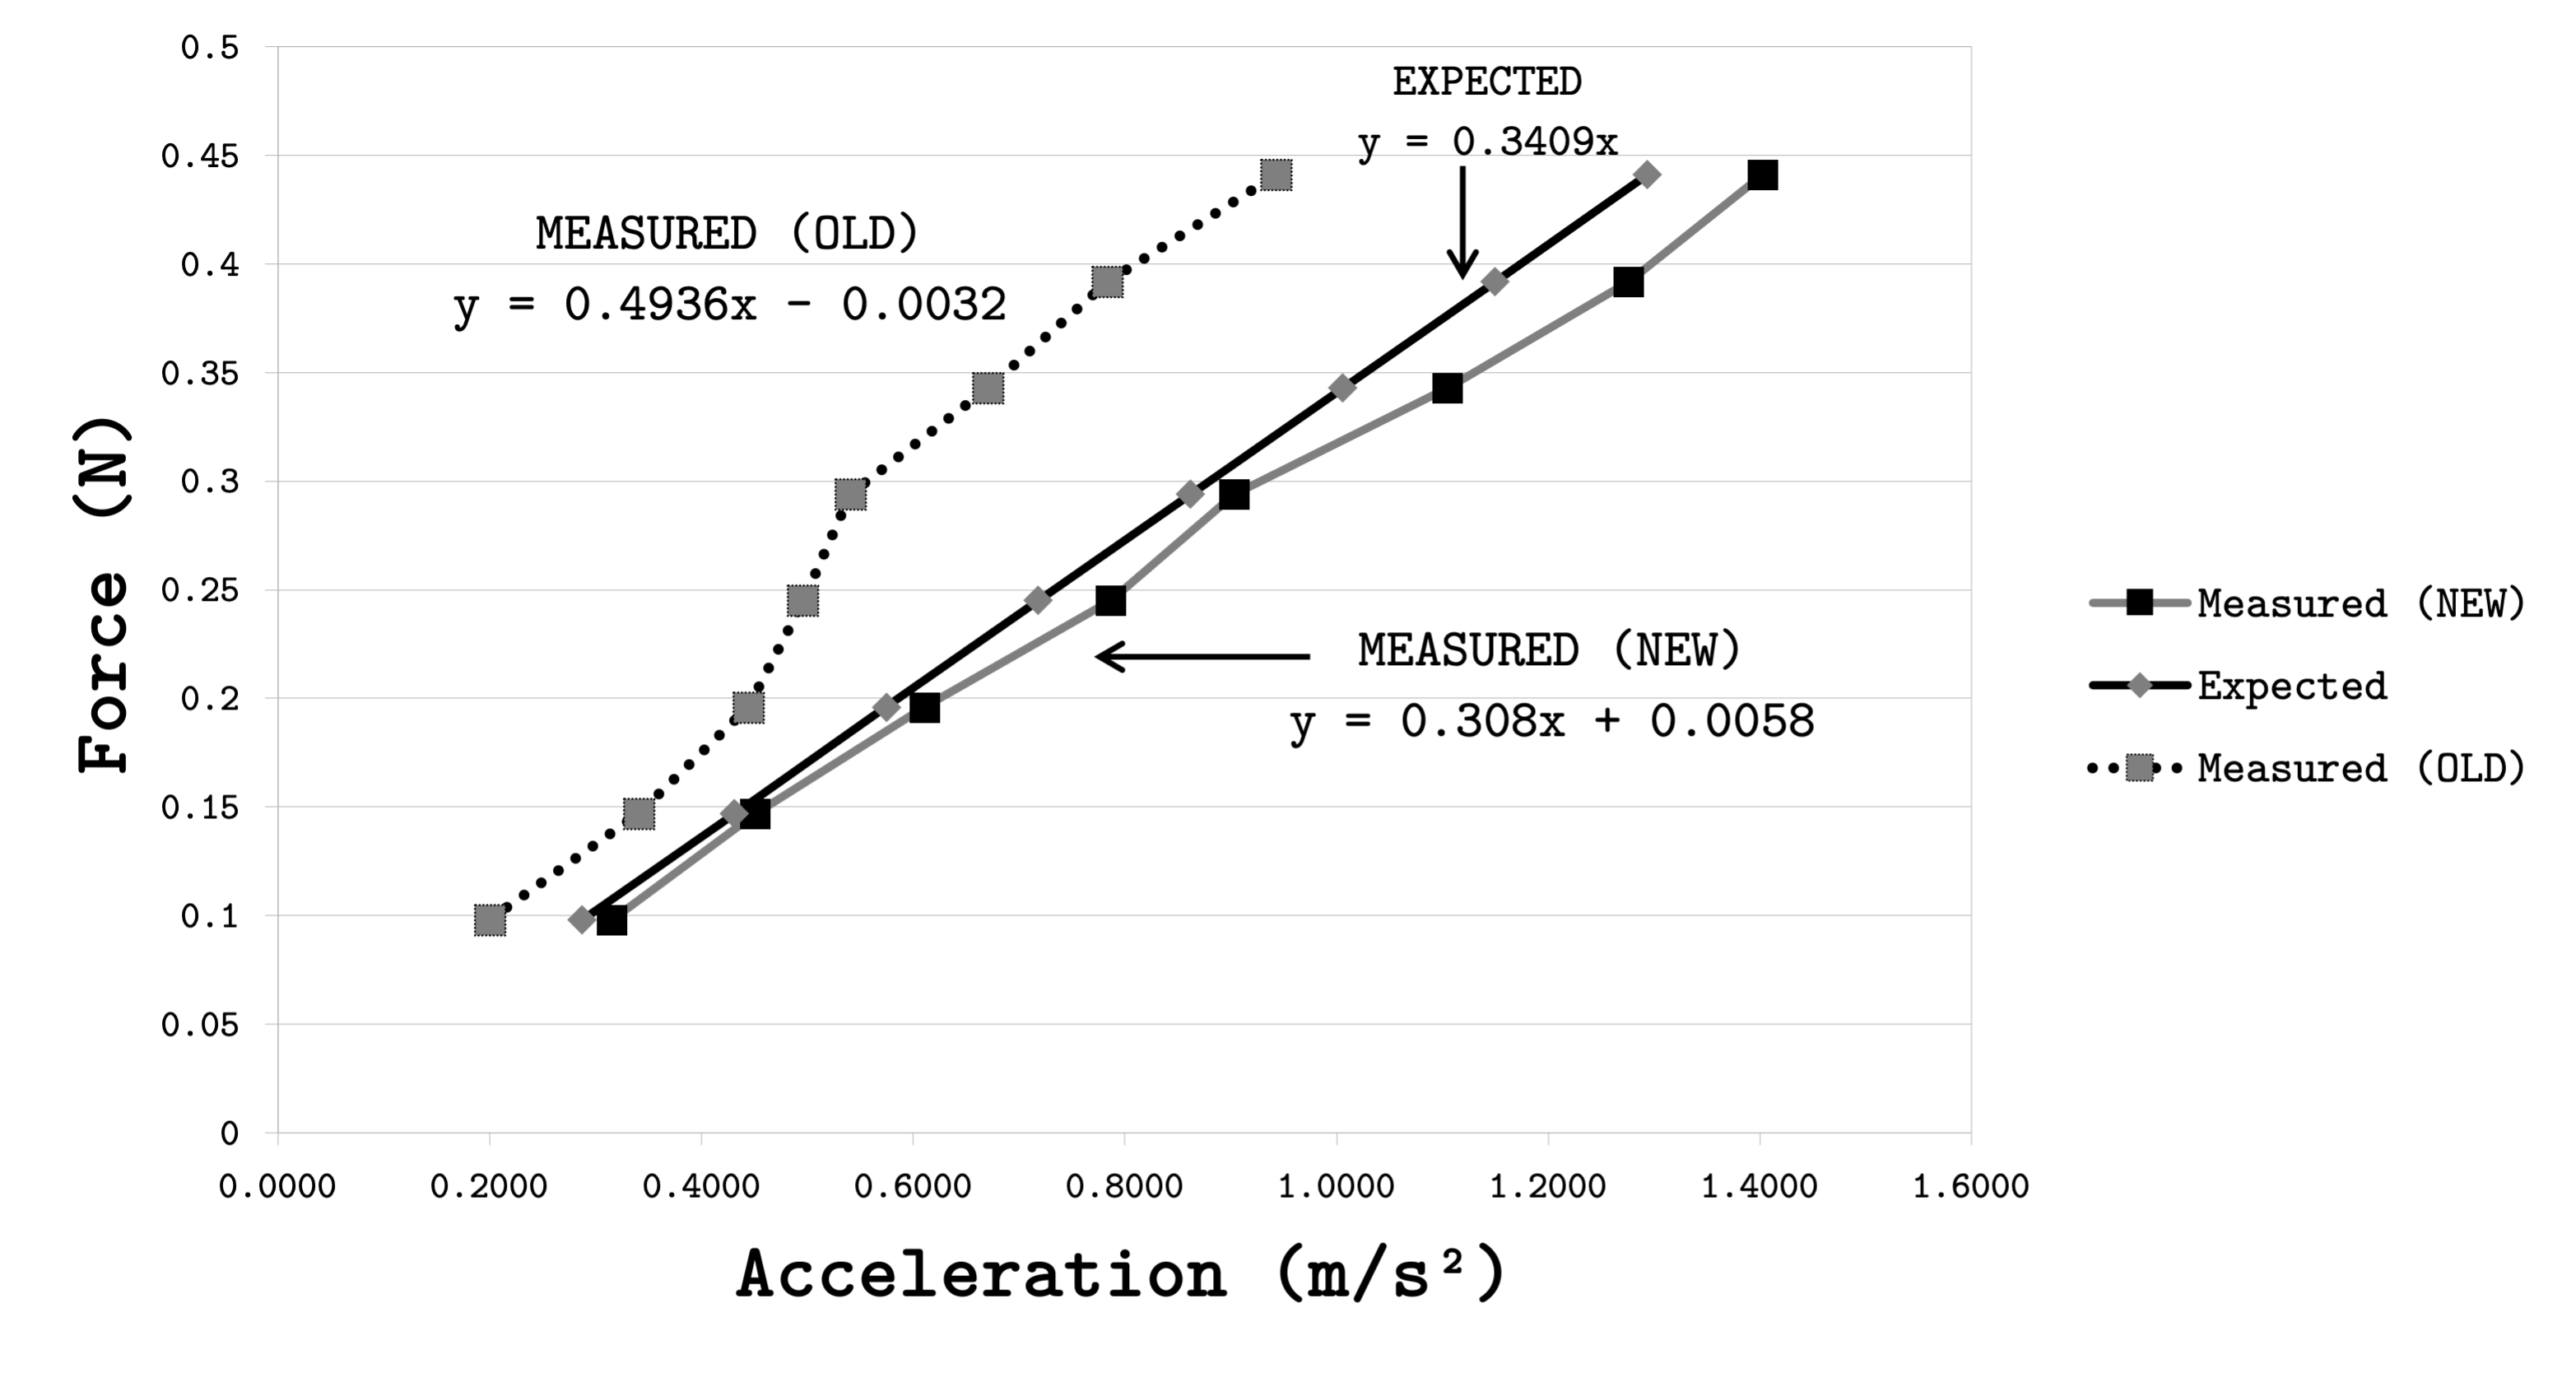
\includegraphics[width=0.90\columnwidth]{images/GraphFvA}
	\end{center}
\end{figure}
\end{landscape}

%----GRAPHS-----%

\newpage



%-----------------------------------------------%

% Questions  %

%-----------------------------------------------%

%
 \section{Questions}

\vspace{-0.5cm}
\singlespacing

\begin{enumerate}
	\item \textbf{What do you expect the acceleration of the picket fence to be? Is it exactly this value? If yours is higher or lower provide explanations as to why that might be.}

		We expected the acceleration of the picket fence to be around $9.80\thinspace{m/s^2}$. Our calculations ended up being slightly slower but well within 10.0\% of difference. The difference in values could be due to air resistance, or the small breeze produced by multiple bodies moving at the same time in a room.

	\item \textbf{Do you expect that the detector's measurement of time is exactly correct? What might affect the detector's measurement of time?}

	The detector itself has a few seconds of delay so the measurement of time wouldn't be completely accurate. It's also possible that the detection algorithm of the device is finely tuned such that the minute blending of colors at the borders on the picket fence would cause times to be off. The angle at which the picket fence was dropped could also have affected the Photogate's readings.

\item \textbf{What is your average value, standard deviation, and relative error for the acceleration due to gravity, \textit{g}?}

		For the acceleration due to gravity, \textit{g}, our average value was \textbf{$9.747\thinspace{m/s^2}$}, our standard deviation was \textbf{$0.06439\thinspace{m/s^2}$}, and the relative error was .5408\%.

\item \textbf{Would dropping the Picket Fence from higher above the Photogate timer change the measured value of g? Explain.}

	Dropping the Picket Fence from higher above the Photogate timer should not change the measured value of g by any significant amount. The measured value of g should change incredibly slightly since it's being dropped from a distance that is slightly farther from the Earth's surface.

\item \textbf{Does the acceleration found from the velocity vs time graphs in section 2.2 and 2.3 match each other? Should they be similar? Explain.}

	The acceleration found from the velocity vs time graphs in section 2.2 and 2.3 \textit{do} match other. The accelerations should be similar since no part of the track has been changed (angle and height is the same). The biggest source of difference between the graphs should be because of the cart being pushed up to the top of the track in 2.3, as opposed to being let go from it in 2.2. From the point where the cart starts coming back down in 2.3, the acceleration should be similar to 2.2, which the data shows. 

\item \textbf{Using $a=gsin\theta$ and $9.8\,m/s^2$ as the accepted value of g, calculate what you should have gotten from the motion detector for the acceleration along the ramp. Compare this value with the average value you found for the cart moving down the ramp and the average from the up and down the ramp. Is it within 10\% error?}

	After our calculations, the value that we should have gotten from the motion detector for the average acceleration along the ramp was -0.6105\,$m/s^2$. While our average for starting from the top of the track had a relative error of 12.9\%, our average for starting from the bottom had a relative error of 7.567\%. 
	
\end{enumerate}



%-----------------------------------------------%

		% Conclusion %

%-----------------------------------------------%


\section{Conclusion}

\vspace{-0.5cm}
\singlespacing

The purpose of this lab was to use static equilibrium to solve for the center of mass of a rigid rod. By using a meter stick as our rigid rod, and balancing it on a knife edge, we were able to experimentally and through calculation, determine not only its center of mass, but also what positions to place masses on it and maintain static equilibrium. First, we experimentally found the meter stick's center of mass to be 0.509 m (see Table~\ref{tab:s1tab}). Then we placed a 60 g mass 20 cm from one end of the meter stick, applying a torque on that side (see Figure~\ref{fig:Scenario1}). Next we experimentally determined the position to place a 100 g mass to the left of the meter stick's pivot such that the net torque on the meter stick was 0 (see Figure~\ref{fig:Scenario1}). Through experimentation, we determined the position of the 100 g mass to balance the meter stick, to be at 0.333 m on the meter stick (see Table~\ref{tab:s1tab}). Since torque decreases the closer an object is to the pivot point, it makes sense that in order to balance out the torque of the 60 g mass on the other side, the 100 g mass was closer to it than the 60 g mass. Using equation ~\ref{eq:COM} and rearranging it to solve for the expected position of the 100 g mass, we found there to be a 0.4186\% difference with our measured value. 

In the next scenario, we had results that differed a bit from our calculations. We added a 20 g mass to the same side as the 60 g mass, and through experimentation, found the position to place the 100 g mass to be at 0.19 m on the meter stick. Using equation ~\ref{eq:COM}, we found the expected position of the 100 g mass to be 0.2322 m, which is an 18.17\% difference from our measured value (see Table~\ref{tab:s2tab}). Considering that the expected value is closer to the pivot, it's possible that the 20 g mass, and its mass holder, were greater than we thought. Since torque increases the further an object is from the pivot (see ~\ref{eq:torque}), the 100 g we measured was applying a greater torque than the expected value (see Table~\ref{tab:s2tab} and equation~\ref{eq:torque}). This suggests that either the 20 g mass and mass holder were more than 20 g, or the positions of them masses were farther away from the pivot than we recorded. Were I to repeat this experiment again, I would measure the weight of the mass holders as well and ensure that each mass is tightly attached to the meter stick to minimize as much potential sliding as possible. 

In scenario 3 we removed all masses from the meter stick and attached only a 50 g mass, 30 cm from one end of the meter stick. This time we did not add a counter balancing mass to the other end, so we needed to change the meter stick's center of mass. By equation~\ref{eq:torque}, the further an object is from the pivot point, the greater torque it applies. The uniform rod then becomes non uniform, and its distribution of mass unequal. Therefore, to reduce the torque of the 50 g mass, we needed to shift the meter stick's center of mass. Through experimentation we, found that shifting the pivot of the meter stick to 0.6 m, 10 cm behind the 50 g mass, balanced the it (see Figure~\ref{fig:Scenario3}). Using equation~\ref{eq:COM}, we found the expected center of mass to be 0.5833 m, which is only a 2.857\%  from our measured center of mass (see Table~\ref{tab:s3tab}).


\end{document}



